\chapter{Übungen}\label{app:A_Übungen}

\section{Einleitung}

\section{Statik 2}

\underline{Aufgabe 2.0.1}

\begin{minipage}{.58\textwidth}
    Drei Kräfte wirken auf den Körper.
    Das Mass $a$ ist $2m$.
    Zu bestimmen ist das Moment der Kräfte bezüglich
    dem Punkt $A$ sowie die Lagerkräfte $A_x$ und $A_y$.
    $F_1 = F_2 = F_3 = 10N$ (8)
\end{minipage}
\hspace{.1\textwidth}
\begin{minipage}{.3\textwidth}
    \begin{figure}[H]   
        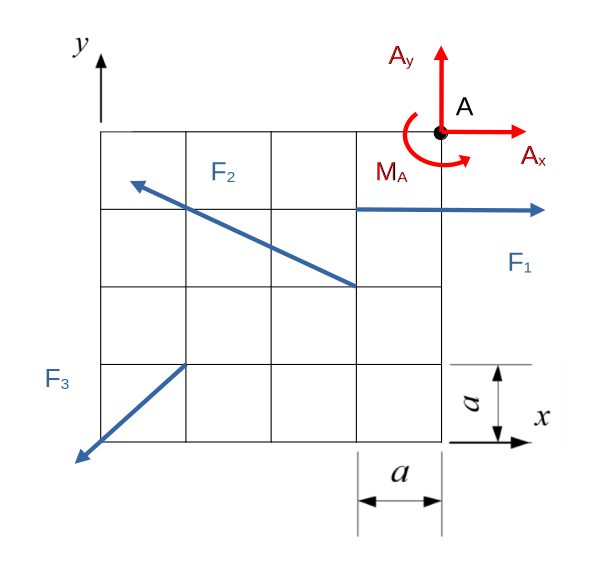
\includegraphics[width=\textwidth]{images/aufgabe_201.png} %.6 stands for 0.6 x textwidth
    \end{figure}
\end{minipage}

\underline{Aufgabe 2.0.2}

\begin{minipage}{.58\textwidth}
    An einem Hebel greifen 3 Kräfte an. \newline
    Es sind die auf die Welle 0 wirkende resultierende Kraft nach Betrag
    und Richtung und das resultierende Moment zu berechnen.
\end{minipage}
\hspace{.1\textwidth}
\begin{minipage}{.3\textwidth}
    \begin{figure}[H]    
        \centering          %     left botm right top
        \includegraphics[clip, trim=0cm 0cm 0cm 0cm,width=\textwidth]{aufgabe_3_3_3_1.png} %.6 stands for 0.6 x textwidth
        \label{fig:3331}
    \end{figure}
\end{minipage}

\underline{Aufgabe 2.1.1}

\begin{minipage}{.58\textwidth}
    Ein Balken der Länge $l = 2m$ ist im Festlager $A$ (links) und im Loslager $B$
    (rechts) gelagert. Auf ihn wirken die vertikalen Kräfte $F = 300N$ im Abstand
    $0.5m$ von $A$ sowie $G = 100N$ in Balkenmitte. Am rechten Ende greift zusätzlich
    die horizontale Kraft $F_h = 50N$ an. \newline
    Zu bestimmen sind die Lagerreaktionen $A_x$, $A_y$ und $B$ sowie die
    dimensionierende Lagerkraft $A$.
\end{minipage}
\hspace{.05\textwidth}
\begin{minipage}{.35\textwidth}
    \begin{figure}[H]   
        \includegraphics[width=\textwidth]{aufgabe_2_1_1.png}
    \end{figure}
\end{minipage}

\underline{Aufgabe 2.1.2}

\begin{minipage}{.58\textwidth}
    Zu bestimmen sind die Seilkraft und die 
    Auflagerreaktion in A.
\end{minipage}
\hspace{.1\textwidth}
\begin{minipage}{.3\textwidth}
    \centering
    \includegraphics[width=\linewidth]{aufgabe_2_1_2.png}
\end{minipage}